\documentclass{article}
\usepackage{hyperref}
\usepackage{rotating}
\usepackage{multirow}
\usepackage{amsmath}
\usepackage{geometry}
\geometry{letterpaper,tmargin=2.54cm,bmargin=2.54cm,lmargin=2.54cm,rmargin=2.54cm} 


\begin{document}

\title{Homework 2 - Association Statistics and Power}

\author{COMSCI/HUMGEN 124/224}

\date{Due: April 21st, 2017, 11:55 pm}

\maketitle

This short programming assignment is designed to help you get an
understanding for the basics of power and association computations
from a computational perspective. You can use any language
for this project, though Python and R are recommended. You will
need to submit your code along with your results file through CCLE.


\section*{Association Study at a Single SNP}

\subsection*{Reading the input}
The data for this programming assignment consists of a matrix
of 2,000 individuals, 100,000 SNPs, and one column representing
the individual's status as a case or control. Unzip the file \verb!SNP_status.zip!,
and you'll see a space-separated text file.
Each column of the input represents a single SNP, and each row
represents an individual. Each element in the matrix represents
the number of copies of a single SNP an individual has.

To get started, you may want to look at the documentation for
the Python module \verb!pandas read_csv! function,
or the documentation of R's \texttt{read.table} function.

If you aren't sure where that is, literally copy and paste
the module and method you're into Google. That trick
increases beginning computer 
programmer productivity by about 50 percent.


\subsection*{Part A - Computing Association Statistics}
Your job will be to compute the association statistic, the non-centrality
parameter, and the corresponding p-value for each SNP.
s
You should use the formulas that we have developed in
class to compute association statistics.  Use the statistic:

$$ S_A = \frac{\hat p^+_A - \hat p^-_A}{\sqrt{2/N}\sqrt{\hat p_A(1 - \hat p_A)}} \sim N(0,1)$$

Once you have the association statistic, use the normal
quantile function to compute p-values. \textbf{Use a two-tailed test for
significance; report the p-values as described in Part D.}


\subsection*{Part B - Bonferroni Correction}
Bonferroni correction is a way to maintain the "family-wide error rate"
(FWER) of a set of related tests.
If we want perform $m$ tests of significance level $\alpha$ on 
data that conform to the null hypothesis, we would expect to find $m\alpha$ tests
passing that level of significance on average, under the null.  When $m$ is large
To combat this, we make each test pass a more
stringent threshold of $\frac{\alpha}{m}$.

For this assignment, use $\alpha = .05$ for your two-tailed test. That is, 
a test is considered significant if and only if it is within the upper
or lower 2.5\% tails of the standard normal distribution.

\textbf{Apply Bonferroni correction to your results from Part A
and report the significantly-associated SNPs as described in Part D.}

\vspace{1.5 cm}

\subsection*{Part C - Q-Q plots and Inflation Statistics (Optional for Undergrads, Required for Grads)}
Recall that a p-value is the probability that an association statistic
of a particular magnitude will appear in the data. Given that definition,
we should expect that only 30\% of the individual hypotheses
that we test should have p-values should be stronger than .3. 
If we see more than 30\% of our statistics with p-values stronger than .3,
that indicates our statistical test may be detecting many false positives.

However, it is often the case that we see tests with significantly
increased or decreased p-values with versus our expectation. One way
that this increase or decrease is quantified is using 
a statistic called $\lambda_{gc}$, or the genomic control statistic.

$$\lambda_{gc} = \frac{\text{Median empirical } \chi^2 \text{ statistic}}{\text{Median value of }\chi^2_1 \text{ distribution}}$$

Using Python or R, find the median value of the chi-square ($\chi^2$) distribution 
with one degree of freedom.  You can compute ($\chi^2$)-distributed statistics
by squaring the statistics you generated in Part A.

\textbf{Compute $\lambda_{gc}$ for your study, and report it as described in part D.}

There are many tutorials on how to make a Q-Q plot online;
if you are new to Python or R plotting, it is recommended that you adapt
code from one of these to suit this purpose.  If you're stuck,
Google "QQ Plot R" or "QQ Plot Python" and read the documentation and tutorials.

There are several ways to make a Q-Q plot; what they all have in common
is that the x-value is the expected value of a statistic for a particular quantile,
and the y-axis is the experimental value of the statistic at that quantile.
\begin{figure}[ht]
\begin{center}
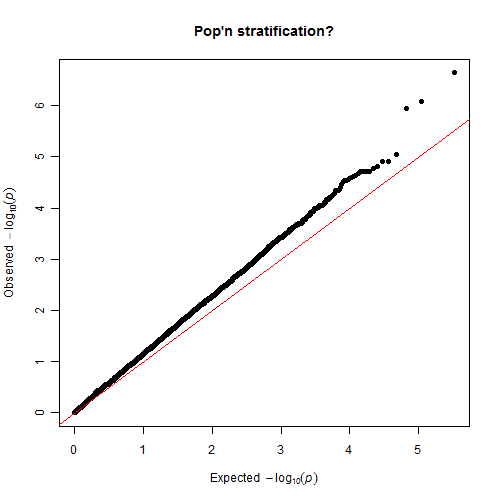
\includegraphics[scale=.4]{qq_example.png}
\end{center}
\caption{A Q-Q plot of p-values, from \url{http://www.gettinggeneticsdone.com/2011/04/annotated-manhattan-plots-and-qq-plots.html}}
\end{figure}

Some statistics you can use include your $S_A$ statistics from part A, which
are distributed as a standard normal under the null hypothesis, the $\chi^2$ statistics
you computed to compute $\lambda_{gc}$, which are distributed as a 
chi-square with one degree of freedom under the null, and the p-values, which
should be distributed uniformly between 0 and 1 under the null. If you use p-values,
it is generally more informative to show their negative log base 10.
If you show the raw p-values, we will not be able to see the interesting 
very small p-values, since their numerical values will be clustered around 0.

\textbf{Make an image of a Q-Q plot of your data and post it in the forums. Try to explain any trends you see.}

\clearpage
\subsection*{Part D - Output Format}
The most important part of this assignment is that you
input and output data in the proper format. The first line
should be your UID; it is recommended that you also put
your UID in the title of your file, but it's not required.

\begin{verbatim}
UID:{Your UID}
email:{Your email}
Undergrad or Grad:{Grad if you're a graduate student, undergrad otherwise}
<A>
{SNPNAME}:{RAW-P-VALUE}
{SNPNAME}:{RAW-P-VALUE}
{SNPNAME}:{RAW-P-VALUE}
...
</A>
<B>
{SIGNIFICANT-SNP1}
{SIGNIFICANT-SNP2}
...
</B>
<C>
Lambda_gc:<Lambda Value>
</C>
\end{verbatim}

If I were to submit an assignment, my output
would look something like this:

\begin{verbatim}
UID:123456789
email:bilow@cs.ucla.edu
Undergrad or Grad:Grad
<A>
SNP0000:0.175
SNP0001:0.875
SNP0002:0.0003
...
</A>
<B>
SNP0002
...
</B>
<C>
Lambda_gc:1.872
</C>
\end{verbatim}


\clearpage




\end{document}
